\documentclass{standalone}

%----------------------------------------------------------------------------------------------%
%                                 Packages and basic declarations
%----------------------------------------------------------------------------------------------%

\usepackage[utf8]{inputenc}
\usepackage{pgfplots}
\usepackage{tikz}


%----------------------------------------------------------------------------------------------%
%----------------------------------------------------------------------------------------------%
%                                            DOCUMENT STARTS
%----------------------------------------------------------------------------------------------%
%----------------------------------------------------------------------------------------------%

\begin{document}


%Tikz picture starts%

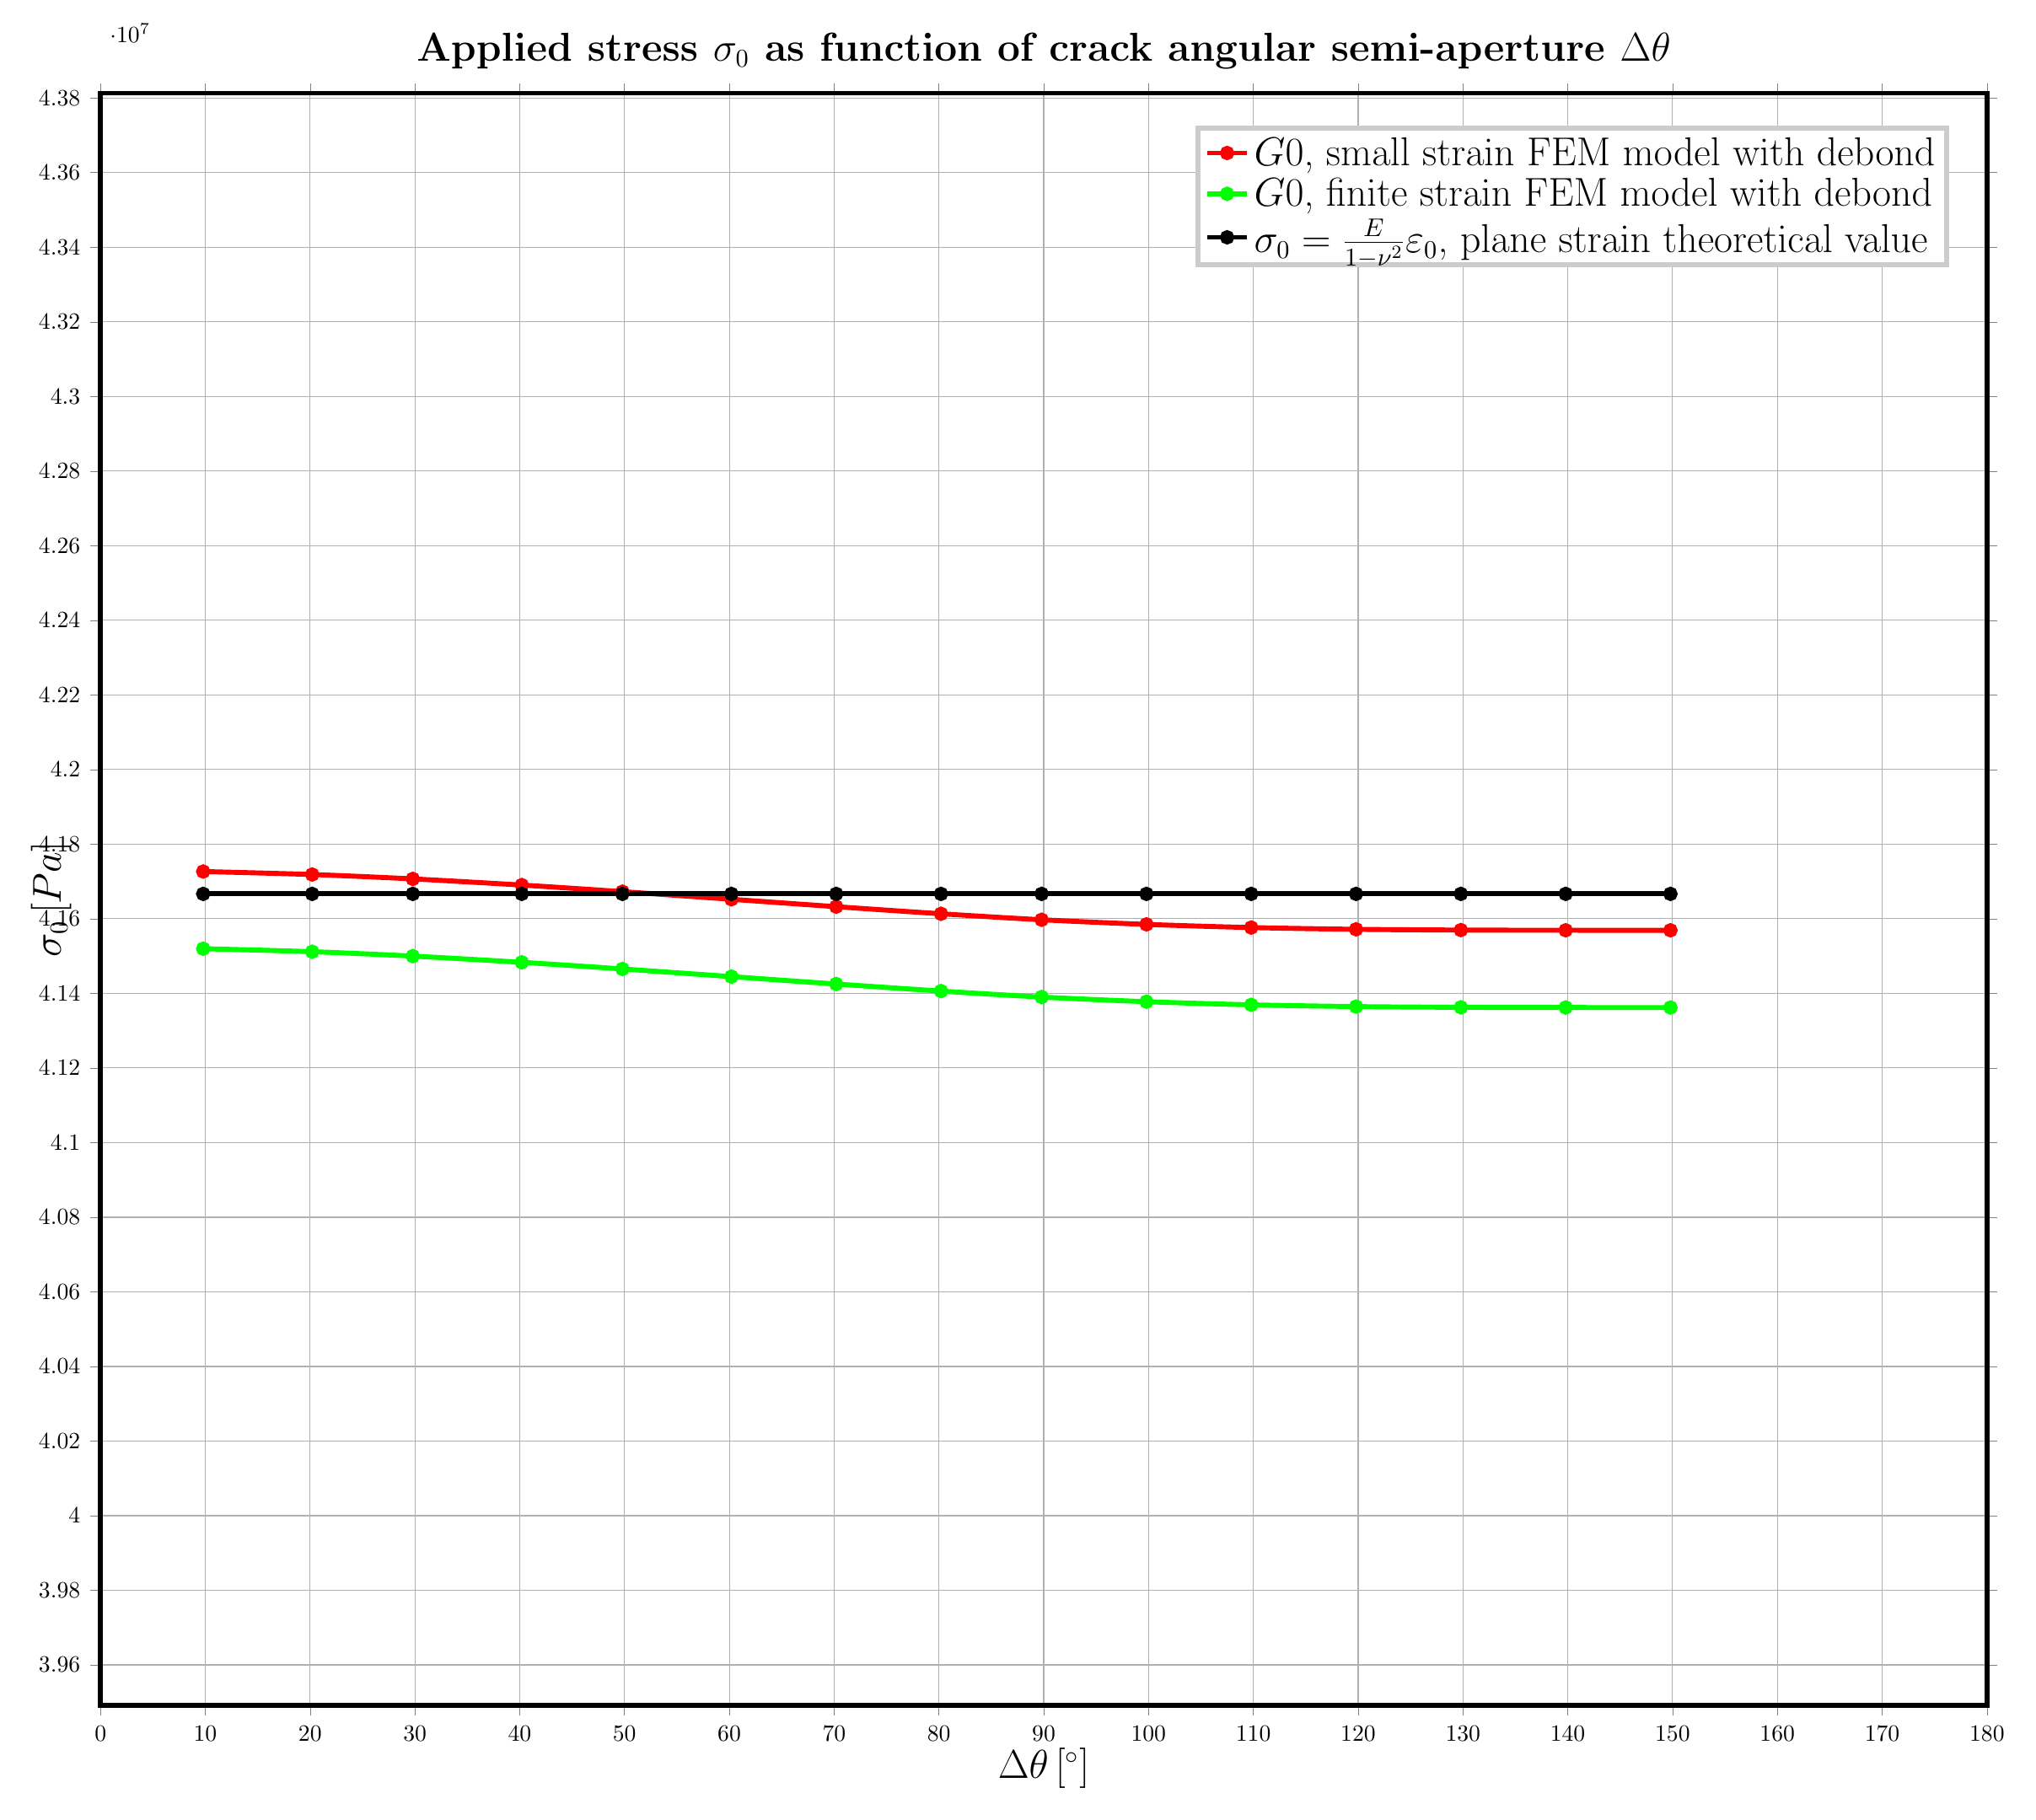
\begin{tikzpicture}

%Tikz axis starts%

\begin{axis}[width=30cm,
title={\bf{Applied stress $\sigma_{0}$ as function of crack angular semi-aperture  $\Delta\theta$}},
title style={font=\fontsize{16}{8}\selectfont},
xlabel style={at={(axis description cs:0.5,-0.02)},anchor=north,font=\fontsize{16}{8}\selectfont},
ylabel style={at={(axis description cs:-0.01,.5)},anchor=south,font=\fontsize{16}{8}\selectfont},
xlabel={$\Delta\theta\left[^{\circ}\right]$},ylabel={$\sigma_{0}\left[Pa\right]$},
xmin=0.0,
xmax=180.0,
ymin=39490679.7164,
ymax=43812938.6104,
tick align=outside,
tick label style={font=\tiny},
xtick={0.0,10.0,20.0,30.0,40.0,50.0,60.0,70.0,80.0,90.0,100.0,110.0,120.0,130.0,140.0,150.0,160.0,170.0,180.0},
xmajorgrids,
x grid style={lightgray!92.026143790849673!black},
ymajorgrids,
y grid style={lightgray!92.026143790849673!black},
tick label style={font=\normalsize},
line width=0.75mm,
legend style={draw=white!80.0!black,font=\fontsize{16}{12}\selectfont},
legend entries={{$G0$, small strain FEM model with debond},{$G0$, finite strain FEM model with debond},{$\sigma_{0}=\frac{E}{1-\nu^{2}}\varepsilon_{0}$, plane strain theoretical value}},
legend cell align={left}
]

\addplot[red,smooth,mark=*]
table{
9.8000083551 41726608.2004
20.2001564043 41718577.9757
29.7996713865 41706819.2896
40.1999526243 41690319.8293
49.8000464651 41672674.8036
60.2003242878 41652209.2228
70.1998714969 41632364.8638
80.1999924418 41613382.0441
89.799994075 41597326.8484
99.8000057369 41584929.4578
109.800126682 41576448.6347
119.799673891 41571731.6518
129.800136345 41569718.8166
139.800052385 41569180.2607
149.799859141 41569136.5436
};

\addplot[green,smooth,mark=*]
table{
9.8000083551 41519773.9221
20.2001564043 41511721.822
29.7996713865 41499885.8798
40.1999526243 41483242.9717
49.8000464651 41465460.7013
60.2003242878 41444920.1179
70.1998714969 41425124.0165
80.1999924418 41406171.2755
89.799994075 41390121.8186
99.8000057369 41377746.9703
109.800126682 41369301.6947
119.799673891 41364617.5756
129.800136345 41362623.6029
139.800052385 41362092.0012
149.799859141 41362049.8117
};

\addplot[black,smooth,mark=*]
table{
9.8000083551 41666666.6667
20.2001564043 41666666.6667
29.7996713865 41666666.6667
40.1999526243 41666666.6667
49.8000464651 41666666.6667
60.2003242878 41666666.6667
70.1998714969 41666666.6667
80.1999924418 41666666.6667
89.799994075 41666666.6667
99.8000057369 41666666.6667
109.800126682 41666666.6667
119.799673891 41666666.6667
129.800136345 41666666.6667
139.800052385 41666666.6667
149.799859141 41666666.6667
};

\end{axis}
%Tikz axis ends%


\end{tikzpicture}
%Tikz picture ends%


\end{document}

%----------------------------------------------------------------------------------------------%
%----------------------------------------------------------------------------------------------%
%                                            DOCUMENT ENDS
%----------------------------------------------------------------------------------------------%
%----------------------------------------------------------------------------------------------%

